\chapterOrPart{Software}\label{ch:Software}

\section{Micropython}
  One of the reasons we choose to work with a development board from pycom was the integration with micropython. Micropython is a lightweight, open source version of python that runs well on low power devices. All you need is a python file and the Pymakr extensions to upload the code and you're good to go. 

  The code gets uploaded to /flash on the development board.
  The 2 most important files are boot.py and main.py which are run automatically at boot. Besides these, you can choose the file structure. They do give you some empty folders to help. boot.py and main.py are 2 normal python files which can contain any code. If you want, you can run your entire software in boot.py. Ofcourse, this is not a good way to code which is why we will separate our code into the correct files.

\section{code}
  \subsection{boot.py}
    Lets start off by taking a look at the boot file in \Cref{list: boot}. This is the first file that will be ran on the development board.

    \begin{frame}[fragile]{Listings of code can be easily formatted and displayed}
        \begin{lstlisting}[language=Python, caption={Boot.py},label={list: boot}]
        # Message to indicate the start of the boot file
        print("\n\n\nStarting up fipy")

        # Turn off default flashing LED
        pycom.heartbeat(False)

        # Custom flashing LED
        pycom.rgbled(0xFF0000)  # LED Red
        time.sleep(1)           # wait 1 second
        pycom.rgbled(0x000000)  # LED Off

        # initialize spi communication and CS pin
        spi, cs = spi_init()

        # write the correct configuration to the ADC
        write_config(spi, cs)

        # Message to indicate the end of the boot file
        print("BOOT COMPLETE")

        \end{lstlisting}
    \end{frame}

    Our boot file does several things: 
    \begin{itemize}
        \item print message to indicate the start of the boot file
        \item turn of the default flashing LED
        \item custom flash the onboard LED to visually indicate the start of the boot file
        \item initialize the SPI communication
        \item write the correct configuration to the ADC over SPI
        \item print message to indicate the end of the boot file
    \end{itemize}

    The boot file calls two external functions, spi\textunderscore init and write\textunderscore config. These functions are defined in ADC.py which contains all the functions to interact with the ADC.
    Inside spi\textunderscore init which can be seen at \Cref{list: spi init} we initialize the \pcs\ pin and SPI on the development board with the correct pins and baudrate. We return the spi connection and the \pcs~pin so they can be used.



    \begin{frame}[fragile]{Listings of code can be easily formatted and displayed}
        \begin{lstlisting}[language=Python, caption={Python function to initialize everything required for SPI communication},label={list: spi init}]
        
        def spi_init():
            # INIT PINS
            cs = Pin(PIN_CS, mode=Pin.OUT, value=1)

            # INIT SPI
            spi = SPI(1)
            spi.init(mode=SPI.MASTER, baudrate=9_830_400,
                    pins=(PIN_SCK, PIN_MOSI, PIN_MISO))

            return spi, cs
        \end{lstlisting}
    \end{frame}


    After having initialized the spi communication, we use it to write the correct configuration to the ADC. This function can be seen in \Cref{list: write config}. Before going over the function we first need to know how we communicate using SPI.




    The first thing we do is send a command byte. This is always the first byte that is send after releasing \pcs. 
    The command byte follows the structure shown in \Cref{fig: command byte structure}. 

    \begin{figure}[!ht]
        \centering
        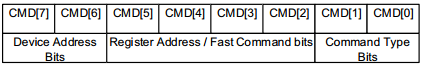
\includegraphics[scale=0.6]{figs/command_byte_structure.png}
        \caption{command byte structure, source \cite{MCP34612020}.}
        \label{fig: command byte structure}
    \end{figure}

      The first 2 bits specify the device address. This is a hardcoded value which depends on the component. For the MCP3461 this value is 01.

      The following 4 bits depend on the last 2 bits as can be seen in \Cref{fig: command byte}. The last 2 bits specify the type of command. There are 4 types: fast command, static read, incremental write and incremental read. fast command is a way of configuring the ADC with only 1 byte. The exact command is specified by the 4 middle bits. All other types require additional bytes to be send. static read is used to continuously read 1 register specified by the 4 middle bits. incremental read/write automatically increase the register pointer after every operation and start at the specified register. 

      \begin{figure}[!ht]
        \centering
        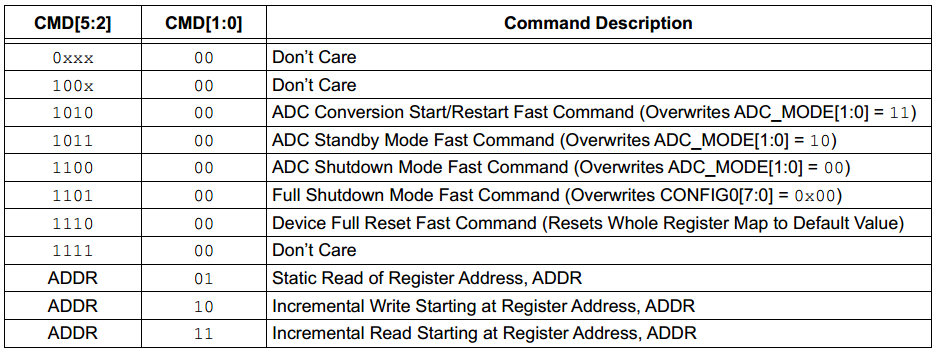
\includegraphics[scale=0.435]{figs/command_byte_bits.png}
        \caption{command byte}
        \label{fig: command byte}
      \end{figure}

      It is important to note that incremental write and incremental read don't follow the same sequence of registers. While incremental read will go over all 16 registers, incremental write will not go over the first register and the last 2 registers. This is because you never have to write to these registers.

      \begin{frame}[fragile]{Listings of code can be easily formatted and displayed}
        \begin{lstlisting}[language=Python, caption={write\textunderscore config function},label={list: write config}]

        # REGISTER VALUES
        CONFIG0 = 0xE2
        CONFIG1 = 0x00
        CONFIG2 = 0xA3
        CONFIG3 = 0xC1
        IRQ = 0x77
        
        def write_config(spi, cs):
            print("WRITING SETUP VALUES TO REGISTERS")
            buff = bytearray(1)  # buffer to store responses in
            cs(0)  # Start communication

            # send command byte, store response in buff
            spi.write_readinto(bytes([0x46]), buff)
            print("Response command byte: ", hex(buff[0]))
        
            spi.write(bytes([CONFIG0]))  # CONFIG0
            spi.write(bytes([CONFIG1]))  # CONFIG1
            spi.write(bytes([CONFIG2]))  # CONFIG2
            spi.write(bytes([CONFIG3]))  # CONFIG3
            spi.write(bytes([IRQ]))  # IRQ
            spi.write(bytes([0x08]))  # MUX
            spi.write(bytes([0x00]))  # SCAN
            spi.write(bytes([0x00]))
            spi.write(bytes([0x00]))
            spi.write(bytes([0x00]))  # TIMER
            spi.write(bytes([0x00]))
            spi.write(bytes([0x00]))
            spi.write(bytes([0x00]))  # OFFSET CALIBRATION
            spi.write(bytes([0x00]))
            spi.write(bytes([0x00]))
            spi.write(bytes([0x80]))  # GAIN ERROR CALLIBRATION
            spi.write(bytes([0x00]))
            spi.write(bytes([0x00]))
            spi.write(bytes([0x90]))  # RESERVED
            spi.write(bytes([0x00]))
            spi.write(bytes([0x00]))
            spi.write(bytes([0x50]))  # RESERVED
            # LOCK (Anything except A5 locks all register values)
            spi.write(bytes([0xA5]))
        
            cs(1)  # End communication

        \end{lstlisting}
    \end{frame}

      Looking at the code in \Cref{list: write config} we can see that when writing the initial configuration we use incremental write mode, starting at register 0x01. The command byte for this action is 0x46.
      Every successful command byte will be responded to with a status byte. The status byte allows us to see certain flags without having to read the IRQ register. The status byte always starts off with two '0' bits to give other devices time to respond to avoid bus contention. The next three bits will confirm the hardcoded device address by repeating it and then adding the reversed last bit. The last three bits are flags for Data ready interrupt, CRC checksum error on the register map interrupt and POR interrupt.

      After having send the command byte, and thus having set the ADC in incremental write mode starting at register 0x01, we start to send the values we want to place in the registers. 

      The datasheet contains a list of all possible configurations for every register. We will only go over the ones we use.

    \subsubsection*{CONFIG0}\label{sss: CONFIG0}
      The first value send is 0xE2 for register 0x01 which is also named CONFIG0. 0xE2 can also be written as 11 10 01 00. This will set 4 different settings.
      \begin{itemize}
        \item bit 7-6: if this value is 00, and all other bits in CONFIG0 are to, the ADC will go into shutdown mode. we set it to 11.
        \item bit 5-4: this determines the selected clock, 10 sets it to use the internal clock and to not show the clock on an output pin.
        \item bit 3-2: 00 is chosen to not add any current source to the ADC input pins.
        \item bit 1-0: 00 is chosen to keep the ADC in shutdown mode until we need to start capturing data.
      \end{itemize}

    \subsubsection*{CONFIG1}\label{sss: CONFIG1}
      After writing 0xE2, the pointer will automatically go to the next register: CONFIG1. This time we send 0x00 or 00 0000 00.
      \begin{itemize}
        \item bits 7-6: 00 specifies a prescaler value for the clock of x1.
        \item bits 5-2: This sets the oversampling ratio. 0000 is equal to a OSR of 32.
        \item bits 1-0: these bits should always be set to 00
      \end{itemize}

      The OSR together with the Digital Master Clock or DMCLK determine the sample rate. The OSR is the value we select in CONFIG1 which in this case is 32. The DMCLK is dependent on the Analog Master Clock or AMCLK. The AMCLK is dependent on the Master Clock or MCLK. In this case we have selected the internal MCLK which is \MHz{4.9152}. To calculate the AMCLK from the MCLK we simple divide the MCLK by a prescaler value which we can select in CONFIG1. In our case this value is 1 so the AMCLK is equal to the MCLK. Now to calculate the DMCLK we divide the AMCLK by 4. This gives us 
      \begin{equation}\label{eq: DMCLK}
        \text{DMCLK} = \frac{\text{AMCLK}}{4} = \frac{\text{MCLK}}{4} = \frac{\MHz{4.9152}}{4} = \MHz{1.2288}.
      \end{equation}

      To determine the data rate we simply divide the DMCLK by the OSR. This gives us
      \begin{equation}\label{eq: data rate}
        \text{Data rate} = \frac{\text{DMCLK}}{\text{OSR}} = \frac{\MHz{1.2288}}{32} = \kHz{38.4}.
      \end{equation}

      As we have seen in \Cref{ss: Sampling} our sampling rate should be at least twice the highest frequency in the signal. with a maximum frequency of 20~kHz we would need a data rate of at least 40~kHz which we don't have in this case. Our data rate is close enough to 40~kHz that it won't cause a lot of problems but it is something to keep in mind. A solution is discussed in \Cref{ch:Future work}.
  
    \subsubsection*{CONFIG2}\label{sss: CONFIG2}
      The next byte send is 0xA3 or 10 100 0 11 to CONFIG2.
      \begin{itemize}
        \item bits 7-6: 10 sets the bias current to x1
        \item bits 5-3: 100 sets the GAIN to x8
        \item bit 2: This bit determines wether the ADC uses a auto-zeroing algorithm. We set it to 0 to disable it.
        \item bits 1-0: These bits should always be set to 11
      \end{itemize}

    \subsubsection*{CONFIG3}\label{sss: CONFIG3}
      The next byte send is 0xC1 or 11 00 0 0 0 1 to CONFIG3.
      \begin{itemize}
        \item bits 7-6: 11 sets the ADC to continuous conversion mode.
        \item bits 5-4: These bits specify the ADC output format. 00 sets the format to 16 bits without allowing overrange.
        \item bit 3: this bit specifies the checksum format. Since we don't use checksums we don't care about this bit. We leave it at its default value  of 0.
        \item bit 2: This bit enables checksum. Setting it to 0 turns it off.
        \item bit 1: this bit enables digital offset calibration. We leave it off by writing a 0.
        \item bit 0: this bit enables GAIN. We set it to 1.
      \end{itemize}

    \subsubsection*{IRQ}\label{sss: IRQ}
      The next register is the interrupt register. We write 0x77 or 0111 0 1 1 1 to it. For the first 4 bits we don't care about the values and just leave them at their defaults.
      We do set the next 4 bits.
      \begin{itemize}
        \item bits 3: specify what data is put on the IRQ/MDAT pin. In this case we choose to output all interrupts.
        \item bit 2: setting this bit to 1 sets the inactivate state of the IRQ pin to logical high.
        \item bit 1: setting this bit to 1 enables fast commands.
        \item  bit 0: setting this bit to 1 enables conversion start interrupt output.
      \end{itemize}

    \subsubsection*{MUX}\label{sss: MUX}
      The next byte we write is to the MUX register which determines what pins to use for Vin+ and Vin-. we write 0x08 or 0000 1000 to this register. This sets Vin+ at ch0 and Vin- at ch1. These are also the default values.

    \subsubsection*{SCAN}\label{sss: SCAN}
      After the MUX register we set the SCAN register. This register has to be set to 0x00 otherwise we will be running the ADC in scanning mode which is not what we want.

    \subsubsection*{Other registers}\label{sss: Other registers}
      After the MUX register we continue to write the default values to the remaining registers to make sure they are set correctly. These registers are TIMER, OFFSETCAL, GAINCAL, RESERVED and RESERVED.

    \subsubsection*{LOCK}\label{sss: LOCK}
      Finally when we have have written the correct configuration we lock the registers by changing the value in the LOCK register to something else then 0xA5 and then we pull \pcs~high to end the spi communication.

      This is the end of the boot.py file and also the beginning of the main.py file.

  \subsection{main.py}
    Inside the main.py file we have a while true loop which runs every 15 minutes. Inside the loop we do the following:
    \begin{itemize}
      \item set the ADC mode to conversion using a fast command
      \item read the ADCDATA register at address 0x00 a total of 512 times. The data is stored in an array.
      \item set the ADC mode to shutdown using a fast command
      \item Calculate the average loudness in dB~SPL
      \item Calculate the FFT of the data
      \item Turn on a green LED for 1 second to indicate a successful loop.
      \item put the device in sleep mode for 15 minutes repeat back from step 1.
    \end{itemize}

    \begin{frame}[fragile]{Listings of code can be easily formatted and displayed}
      \begin{lstlisting}[language=Python, caption={Main.py file},label={list: main}]
      
      if __name__ == "__main__":
        while True:
          FC_conversion(spi, cs) # Put ADC in conversion mode       
          measurements = read_ADCDATA(spi, cs) # Read 512 measurements
          FC_shutdown(spi, cs) # Put ADC in shutdown mode
          
          dB = average_dB(measurements) # Calculate the average dB value
          
          y = dft_ulab(measurements) # Calculate DFT with ulab library

          # Transmit dB and y over LoRa
          # Insert LoRa code here
      
          # Flash LED to indicate a successful routine
          pycom.rgbled(0x00FF00)  # Green # DEBUGGING PURPOSES
          time.sleep(1) # DEBUGGING PURPOSES
          pycom.rgbled(0x000000)  # Off # DEBUGGING PURPOSES
          
          machine.sleep(15 * 60 *1000)
      \end{lstlisting}
    \end{frame}
\section{Data Processing}\label{sec: data processing}
  The captured data is used to calculate 2 things, the loudness in dB~SPL and the frequency spectrum. In the following sections we will explain how we calculate these values.

  \subsection{Calculating the SPL in dB}\label{ss: Calculating the SPL in dB}
    Since the goal of this project is to capture data about sound pollution it is important to correctly calculate the loudness of the sound. To convert the measured analog value to dB~SPL we use the formula
    \begin{equation}
      \label{eq: db}
      \up{  output = 20 \cdot \log_{10} \left( \frac{V_{m}}{V_{ref}} \right)}
    \end{equation}
    where V\textsubscript{m} is the measured voltage and V\textsubscript{ref} is the reference voltage.

    When working with an analog microphone the V\textsubscript{ref} is given for a 1~kHz signal of 94~dB~SPL. We also need to account for the GAIN we add to the signal. This transforms the formula into
    \begin{equation}
      \label{eq: db adjusted}
      \up{output = \dB{94} + 20 \cdot \log_{10} \left( \frac{V_{m}}{V_{ref}} \right) - GAIN}
    \end{equation}

    where the GAIN is the total gain of the system in dB. To use this formula we need to calculate V\textsubscript{m}, V\textsubscript{ref} and the GAIN in dB.

    To calculate V\textsubscript{m} we convert the integer value from the ADC to a voltage. This is done by using the formula
    \begin{equation}
      \label{eq: Vm}
      \up{V_m = (measurement / ADC_{res}) \cdot V_{ref}}
    \end{equation}
    where ADC\textsubscript{res} is the resolution of the ADC which is the highest possible integer value it can output. In our case we have a 16 bits ADC which measure 65536 different values between \num{-32768} and \num{32767}. V\textsubscript{ref} is the reference voltage we choose which is 2.84~V. The measurement is the integer value we get from the ADC.

    This gives us 
    \begin{equation}
      \label{eq: Vm worked out}
      \up{V_m = (measurement / 32768) \cdot 2.84}
    \end{equation}

    To calculate V\textsubscript{ref} we need to know the sensitivity of the microphone. This is the voltage the microphone outputs when it measures 94~dB~SPL. In  \cite{ICS40300} we find that the ICS-40300 has a sensitivity of -45~dBV at 1~kHz, 94~dB~SPL. To convert this value to V we take the reverse logarithm. This gives us
    \begin{equation}
      10^{\dBV{-45}/20} = \V{0.005623}.
    \end{equation}
    In this case \V{0.005623} tells us what the output of the microphone will be for a 1~kHz signal of 94~dB~SPL. If the microphone outputs double this value, \V{0.011246}, we know that the signal is increased by 6~dB and is thus equal to 100~dB~SPL. If the microphone outputs half this value, \V{0.002812}, we know that the signal is decreased by 6~dB and thus 88~dB~SPL.

    Finally we need to convert the GAIN to dB with formula \ref{eq: GAIN}.
    \begin{equation}
      \label{eq: GAIN}
      \up{GAIN = 20 \cdot \log_{10} \left( \frac{V_{out}}{V_{in}} \right)}
    \end{equation}
    In our case we have a GAIN of 8 which gives us
    \begin{equation}
      \label{eq: GAIN worked out}
      \up{GAIN = 20 \cdot \log_{10} \left( 8 \right) = \dB{18.06}}
    \end{equation}

    When we combine V\textsubscript{m}, V\textsubscript{ref} and the GAIN in dB into formula \ref{eq: db adjusted} we get
    \begin{equation}
      \label{eq: db worked out}
      \up{output =  \dB{94} + 20 \cdot \log_{10} \left( \frac{\frac{measurement}{\num{32768}}\cdot 2.84}{\V{0.005623}} \right) - \dB{18.06}}.
    \end{equation}

    



  \subsection{Calculating the DFT}\label{ss: Calculating the DFT}

    Besides knowing the loudness of the sound it is also important to know what frequencies these sounds are at. To know this we have to calculate the Discrete Fourier Transform or DFT. The DFT is not a simple calculation, especially in python it is going to be slow. One way of speeding the calculation up is by using the FFT instead. This is an implementation of the DFT where we avoid repeating certain calculations. This helps speed up the calculation by a lot. However, we are still limited by python which is an easy to use but slow language. The way this is resolved in normal python is by doing the heavy calculations in C in the background. This is the approach libraries like numpy take. We are not working with python, but with micropython. This means that we don't have the same libraries available. While micropython has very few built in libraries we can try to add them manually. However, the development board is still a constrained device with only 8~MB of flash RAM. Numpy needs 64~MB of memory. This means we can't just add numpy to the development board. Numpy is also not a library you can easily dissect and remove the parts you don't need. All of this means we will not be able to use numpy for this project. Instead we will try and implement the DFT ourselves.

    The python code for calculating the DFT can be seen in \Cref{list: DFT}. The code was written by \cite{chenPythonImplementationDFT}.


    \begin{frame}[fragile]{Listings of code can be easily formatted and displayed}
      \begin{lstlisting}[language=Python, caption={DFT method},label={list: DFT}]
      
        def DFT(x):
        N, yr, yi = len(x), [], []
        for k in range(N):
            real, imag = 0, 0
            for n in range(N):
                theta = -k * (2 * math.pi) * (float(n) / N)
                real += x[n] * math.cos(theta)
                imag += x[n] * math.sin(theta)
            yr.append(real / N)
            yi.append(imag / N)
        return yr, yi
  
      \end{lstlisting}
    \end{frame}

    This function returns the real and imaginary part of the DFT. It is an implementation of formula \Cref{eq: DFT}. As stated before, python is not the fastest programming language out there and this is the same for micropython. This function takes around 60~s to calculate the DFT of a signal with 512 samples. While time is not a great concern for us since we only wake up once every 15 minutes, this will also use a lot of power. While we have not gone further into the power usage, a power analyzer can be used to measure the exact power usage of this function. However, the time it took to calculate was already enough to try and find a better solution. Fortunately we are not the only ones who needed a fast way of calculating the DFT in micropython. There is a library called ulab that is a replacement for numpy in micropython. However, this library is not part of the official pycom firmware. In order to add this we would have to create a custom fork of micropython with the necessary integration. Like most things, this has been done before by someone else. \cite{chenPythonImplementationDFT} has created a custom fork of micropython that has the necessary code for pycom boards and the ulab library. In order to use this firmware we follow the pycom guide on how to flash firmware and select the custom file instead. The ulab version of numpy is able to calculate the DFT in 0.02~s. This is a huge improvement over the 60~s it took before. This means we can now calculate the DFT in a reasonable amount of time. The code for calculating the DFT using ulab can be seen in \Cref{list: ulab DFT}.

    \begin{frame}[fragile]{Listings of code can be easily formatted and displayed}
      \begin{lstlisting}[language=Python, caption={ulab DFT method},label={list: ulab DFT}]
      
        def dft_ulab(arr):
        c = ulab.array(arr)
        yr, yi = ulab.fft.fft(c)
        y = []
        for i in range(len(yr)):
            y.append(complex(abs(yr[i]), abs(yi[i])))
        return y

      \end{lstlisting}
    \end{frame}


    Even though we are now able to calculate the DFT in a reasonable amount of time, we still have a problem. As stated in \Cref{s: LoRa and LoRaWAN}, LoRa does not have a great throughput. It is more meant for small packets over long distance. In this case, with 512 samples, the DFT would require us to send 1024 floating point numbers. every number is a total of 24 bytes. We can reduce this number by combining yr and yi in a complex number y. a complex number only takes up 32 bytes. This still means we need to send a total of 512 $\cdot$ 32 bytes which is 16384 bytes. As stated in \Cref{s: LoRa and LoRaWAN}, LoRa can only send for 36~s per hour which means we need a data rate of atleast $16384 * 8 / 36 = 3640~\texttt{bits/s}$. While this is a relatively big number for LoRa it can still be done. It will however limit the amount of times we can send per hour. We planned on measuring every 15 minutes but this would require us to have a data rate of 3640 $\cdot$ 4 = 14560~bits/s which is not possible with LoRa. This means we need to find a more efficient way of transmitting data.    

    Another, simpler option would be to just send the originally measured data, it is an arr of 512 integers. While this will result in a lower amount of data, it comes with some big privacy issues as you are essentially building a network that is constantly recording everything that happens and transmitting it. This is not something we want to do and will probably bring some legal issues with it.

  \subsection{Calibration}
    Now that we can calculate the theoretical dB and DFT values, we need to make sure they are correct. To do this we use the setup in \cref{fig: calibration setup}

    \begin{figure}[H]
      \centering
      \tikzset{every picture/.style={line width=0.75pt}} %set default line width to 0.75pt        

      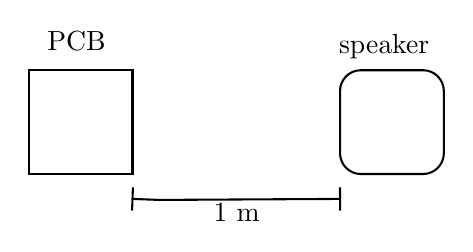
\begin{tikzpicture}[x=0.75pt,y=0.75pt,yscale=-1,xscale=1]
      %uncomment if require: \path (0,105); %set diagram left start at 0, and has height of 105

      %Shape: Rectangle [id:dp182697156127418] 
      \draw   (257,23) -- (307,23) -- (307,73) -- (257,73) -- cycle ;
      %Rounded Rect [id:dp07643316515526455] 
      \draw   (407,33) .. controls (407,27.48) and (411.48,23) .. (417,23) -- (447,23) .. controls (452.52,23) and (457,27.48) .. (457,33) -- (457,63) .. controls (457,68.52) and (452.52,73) .. (447,73) -- (417,73) .. controls (411.48,73) and (407,68.52) .. (407,63) -- cycle ;
      %Straight Lines [id:da684334862272374] 
      \draw    (307,85) -- (319.99,85.49) -- (407,85) ;
      \draw [shift={(407,85)}, rotate = 179.68] [color={rgb, 255:red, 0; green, 0; blue, 0 }  ][line width=0.75]    (0,5.59) -- (0,-5.59)   ;
      \draw [shift={(307,85)}, rotate = 182.16] [color={rgb, 255:red, 0; green, 0; blue, 0 }  ][line width=0.75]    (0,5.59) -- (0,-5.59)   ;

      % Text Node
      \draw (344.57,86) node [anchor=north west][inner sep=0.75pt]   [align=left] {1 m};
      % Text Node
      \draw (264.5,3) node [anchor=north west][inner sep=0.75pt]   [align=left] {PCB};
      % Text Node
      \draw (405,4) node [anchor=north west][inner sep=0.75pt]   [align=left] {speaker};
    \end{tikzpicture}
      \caption{Calibration setup}
      \label{fig: calibration setup}
    \end{figure}

    \Cref{eq: db worked out} is only correct for a perfect microphone. In order to be certain we get accurate dB~SPL measurements we need to calibrate the system. This can be done by using a sound source with a known loudness at a specific frequency and comparing that to what we measure. 
    
    In this case we used a bose soundlink micro speaker which has been analyzed by \cite{panoryiosBoseSoundLinkMicro2023}. According to them, this speaker has a peak loudness of 78.6~dB. We then connect it to a phone and use an app to generate a sine wave of 1~kHz. We then place the speaker at 1~m of the microphone and measure the output. In order to have a more accurate view of the measurements, we repeat it about 20 times and save the results in a text document. We then calculate the average of these measurements and compare them to what we would expect. As previously said, the speaker we use should produce a peak loudness of 78.6~dB. We then subtract this value from the average of our measurements and find a difference of 14.5~dB. This means we need to subtract 14.5~dB from our measurements to get the correct loudness. We then repeat the previous test several more times in order to make sure we have correctly calibrated our system. After repeating the test 4 more times we find that our result is always within 2~dB of what we would expect. While not being the most accurate, this is more then enough for what we are trying to achieve which is finding where in a city we find the most sound pollution.

    This setup can also be used to check the correctness of the FFT calculation. we simply play a sine wave of a certain frequency and compare the output of the FFT to the expected value. We repeat this several times for the same frequency to be sure its consistently correct and the repeat this for different frequencies between 20~Hz and 20~kHz. We find that the FFT gives us an accurate indication of what frequencies are in the signal. 
    
    Since we are using 512 samples for a range of 20~kHz, we have a resolution of 39~Hz. This means that we can only detect frequencies that are at least 39~Hz apart. This is not a problem for us since we are only interested in the general frequency spectrum of the sound and not the exact frequencies.